\begin{frame}{Dataset Exploration \& Processing}
  
\begin{columns}[T]
  \begin{column}{0.55\textwidth}
	\textbf{Data Quality Challenges:}
	\begin{itemize}
	  \item Started with \highlight{6,800 books} from multiple sources
	  \item \textbf{Issues found:}
		\begin{itemize}
		  \item Missing author/category information
		  \item Very short descriptions ($<$ 9 words)
		  \item Inconsistent categorization across sources
		\end{itemize}
	\end{itemize}
	
	\vspace{0.3cm}
	\textbf{Data Engineering Solutions:}
	\begin{itemize}
	  \item \highlight{API enrichment:} OpenLibrary \& Google Books
	  \item \highlight{Quality filtering:} Remove inadequate descriptions
	  \item \highlight{Final dataset:} 5,160 high-quality books
	\end{itemize}
  \end{column}

  \begin{column}{0.4\textwidth}
	\centering
	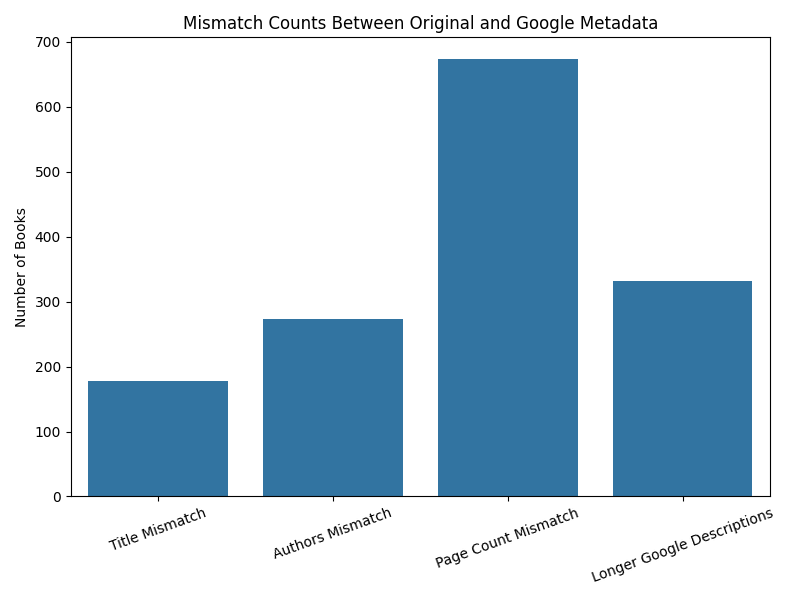
\includegraphics[width=\textwidth]{reexp_mismatch_counts.png}
	
	\vspace{0.2cm}
	\scriptsize \textit{Data inconsistencies across sources required systematic cleaning and validation}
  \end{column}
\end{columns}

\end{frame}

\note{
  \begin{columns}[T]
	\begin{column}{0.49\textwidth}
	  [TIMING: 45 seconds - DATA ENGINEERING STORY:]
	  \begin{itemize}
		\item "Real-world data is always messy - this was no exception"
		\item "Started with 6,800 books but quality varied dramatically" 
		\item "Some books had 2-word descriptions like 'Great book!' - useless for NLP"
		\item "Categories were inconsistent - same book labeled 'Fiction' and 'Novel' and 'Literature'"
	  \end{itemize}
	  
	  \vspace{0.2cm}
	  [EXPLAIN THE CHART (point to it):]
	  \begin{itemize}
		\item "This shows mismatches between original data and Google Books"
		\item "Page count mismatches were highest - shows data quality issues"
		\item "Had to decide: fix manually or filter automatically"
		\item "Chose filtering for scalability"
	  \end{itemize}
	\end{column}
	  
	  \begin{column}{0.49\textwidth}
		[TECHNICAL DECISIONS:]
		\begin{itemize}
		  \item "9-word minimum because shorter descriptions don't contain enough semantic information"
		  \item "API enrichment instead of manual correction - more scalable"
		  \item "25\% data loss acceptable for quality gain"
		\end{itemize}
	  
	  \vspace{0.2cm}
	  [POTENTIAL QUESTIONS:]
	  \begin{itemize}
		\item \textit{"Why not keep all data?"} → "Garbage in, garbage out - quality over quantity for NLP"
		\item \textit{"5,160 seems small?"} → "Proof-of-concept scale, approach scales to millions"
		\item \textit{"How handle missing authors?"} → "API enrichment first, then filtering if still missing"
		\item \textit{"Other data sources?"} → "Could add Goodreads, library catalogs, but these were sufficient"
	  \end{itemize}
	  
	  \vspace{0.2cm}
	  [TRANSITION:]
	  \begin{itemize}
		\item "With clean data, I could focus on the NLP challenge of categorization..."
	  \end{itemize}
	\end{column}
  \end{columns}
}